\section{Skogsbrand}
$\textbf{Delpoäng 1: }$ I den första testfallsgruppen finns bara ett brinnande träd och inga nedhuggna. Det brinnande området kommer att se ut som en "diamant" och innehålla $1,5,13,25,\dots$ punkter för $T = 0,1,2,3,\dots$. Ett sätt att hitta dessa tal är att kolla hur många punkter som finns på varje $x$-koordinat. Vi får då att svaret blir
$$(1 + 3 + 5 + \dots + 2T-1) + 2T + 1 + (2T-1 + 2T-3 + \dots + 3 + 1),$$
förutom för $T = 0$ för då blir svaret $1$. De två summorna inom parenteserna är aritmetiska summor. Om vi grupperar deras termer parvis får vi
$$(1+2T-1) + (3+2T-3) + \dots + (2T-1+1) = 2T + 2T + \dots 2T = 2T^2.$$
Svaret blir alltså $2T^2+2T+1$. Ett annat sätt att komma fram till svaret är att söka på $(1,5,13,25)$ i oeis.org.

En sak att tänka på när man löser den här delgruppen är att se upp med overflows.
Svaret kommer nämligen inte alltid få plats i ett 32-bitarstal. \\

$\textbf{Delpoäng 2: }$ I nästa testfallsgrupp är $M = 0$, $T \leq 100$, och $x_i , y_i < 100$. Det brinnande området kommer se ut som flera "diamanter" som överlappar. Det finns lite olika sätt att lösa de här testfallen. Ett sätt är att simulera spridningen steg för steg. I varje steg kollar vi igenom alla brinnande träd, och markerar de som är bredvid någon av dessa. Eftersom gränserna är så låga borde de flesta såna lösningar klara sig. Ett annat sätt är att notera att de brinnande punkterna är de som är inom Manhattanavstånd $T$ från någon av de givna punkterna. Manhattanavståndet mellan två punkter $(x_1, y_1)$ och $(x_2, y_2)$ definieras som $|x_1-x_2| + |y_1-y_2|$. "Diamanterna" är alltså i själva verket cirklar, Manhattancirklar! Eftersom $T \leq 100$ kommer alla brinnande träd vara inom en $300 \times 300$ ruta, så för att kolla vilka som brinner kan vi loopa igenom alla $300\cdot 300$ punkter och för var och en kolla om Manhattanavståndet till någon av de givna punktera är högst $T$.\\

$\textbf{Delpoäng 3: }$ Den här testfallsgruppen är lite grann en svårare version av den förra. Strategin är att simulera spridningen, men det måste ske på ett ganska effektivt sätt eftersom $T \leq 400$, och vi måste hantera nedhuggna träd. \\

\begin{figure}[!h]
\begin{center}
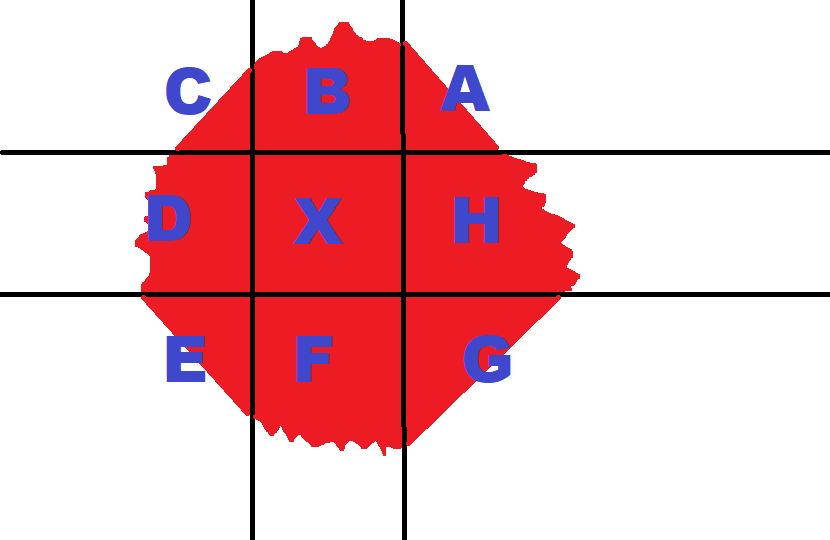
\includegraphics[width=8cm]{skogsbrand_bild.png}
\end{center}
\end{figure}

$\textbf{Delpoäng 4: }$ I den här testfallsgruppen är $M = 0$, $x_i, y_i < 100$, men $T$ kan vara hur stort som helst. Att simulera spridningen i upp till $10^9$ steg är helt uteslutet, vi måste hitta en annan strategi. En viktig observation är att "startområdet" är väldigt litet i jämförelse med $T$. Så efter att elden har spridit sig $T$ gånger kommer startområdet nästan se ut som en punkt, så det brinnande området borde nästan se ut som en Manhattancirkel. Låt oss anta att $T > 200$, om detta inte gäller så hinner vi simulera processen. Dela in planet i $9$ områden enligt bilden. Området $X$ är startrutan, dvs. alla punkter som uppfyller $0 \leq x,y \leq 99$. Eftersom $T > 200$ kommer hela startområdet vara brinnande, så det bidrar med $100\cdot 100$ till svaret. Låt oss se hur mycket de andra områdena bidrar. 
\begin{enumerate}

\item Område $A$ består av alla punkter som uppfyller $x,y \geq 100$. En punkt $(x,y)$ i område $A$ är brinnande om $|x-x'|+|y-y'| \leq T$ för någon av de givna punkterna $(x',y')$. Men $|x-x'|+|y-y'| = (x+y) - (x'+y')$ eftersom $x > x', y > y'$, så vi behöver bara bry oss om den givna punkt som har störst $x'+y'$. Området är alltså en kvartscirkel, och antalet punkter kan beräknas med en aritmetisk summa.

\item Område $B$ består av alla punkter som uppfyller $y \geq 100, 0 \leq x \leq 99$. Låt oss fixera en av dessa $x$-koordinater $x_0$, och se hur mycket $x_0$:s "stapel" bidrar med till svaret. En punkt $(x_0,y)$ i $B$ brinner om $|x_0-x'|+|y-y'| \leq T$ för någon given punkt $(x',y')$. Men $|x_0-x'| + |y-y'| = y + |x_0-x'|-y'$, så vi behöver bara hitta den givna punkt med minst $|x_0-x'|-y'$ för att hitta höjden på stapeln. Vi kan alltså kolla igenom alla $100$ värden på $x_0$, och hitta hur mycket var och en bidrar med.


\end{enumerate}
De andra områdena har samma utseende som $A$ eller $B$ och kan lösas på liknande sätt. \\
Här är en kul alternativ lösning som är svårare att komma på:

\begin{lemma}
    Låt $f(t)$ vara antalet punkter som brinner efter $t$ minuter. Låt oss anta att alla givna punkter är inom avstånd $W$ från varandra i $x$-led, och $H$ i $y$-led (i vårt fall är både $W,H = 100$). Då gäller det att 
    $$f(t+2)-2f(t+1)+f(t) = 4$$
    för alla $t > W+H$.
\end{lemma}
Notera att 
$$f(t+2)-2f(t+1)+f(t) = (f(t+2)-f(t+1))-(f(t+1)-f(t))$$
dvs. "ökningen av ökningen" eller accelerationen om man så vill. Man kan bevisa lemmat genom att kolla på bilden med de nio områdena igen. Område $B,D,F$ och $H$ kommer hela tiden öka med lika mycket, så de bidrar inget till accelerationen. Område $A,C,E,G$ däremot bidrar med $1$ var till accelerationen. \\
Problemet kan nu lösas genom att vi först simulerar i $201$ steg. Därefter beräknar vi $f(200)$ och $f(201)$. Låt $d$ vara $d = f(201)-f(200)$. Enligt lemmat blir nu $f(202) = f(201) + d + 4$, $f(203) = f(201) + d + 4 + d + 8$, osv. Mer allmänt får vi 
$$f(201+t) = f(201) + t\cdot d + 4\cdot (1+2+3+\dots+t) = f(201) + t\cdot d + 2t(t+1).$$
Så nu är det bara att stoppa in $t = T-201$ i formeln och så är vi klara. Svårt att komma på som sagt, men enklare att implementera. \\

$\textbf{Delpoäng 5: }$ Den här delpoängsnivån är samma som den förra fast det kan finnas nedhuggna träd. Lösningen är faktiskt ganska lik den förra också, vi kommer kunna reducera problemet till $M = 0$. Börja med att simulera processen i ungefär $500$ steg. Om de brinnande träden är helt instängda av nedhuggna träd så kommer det märkas, och vi kan bara skriva ut svaret. Annars så kommer elden att omringa alla nedhuggna träd vid det här laget. Vi kan alltså strunta i det inre av brandområdet där alla nedhuggna träd finns, eftersom inget nytt kommer hända där inne. Brandområdet kan nu betraktas som ett stort $(M = 0)$-testfall, och kan lösas med metoden från förra delpoängsnivån. Fast det här området är $1000 \times 1000$ och kan innehålla betydligt fler än $100$ brinnande punkter, så vi måste vara lite mer försiktiga. Ett sätt att hantera det på är att bara kolla på de brinnande punkter som är på kanten av brandområdet. Eftersom det är ca $4000$ såna punkter så borde lösningen till förra delpoängsnivån nu vara snabb nog. \\ Den alternativa lösningen till förra delpoängsnivån fungerar faktiskt här också, om vi simulerar lite fler steg och kollar om träden är instängda. \\

$\textbf{Delpoäng 6: }$ Den här testfallsgruppen kräver bara att $M = 0$. Den är samma som nivå $4$ fast koordinaterna kan vara stora, upp till $10^5$. Om $T \geq 2\cdot 10^5$ så kan vi faktiskt använda exakt samma lösning som i nivå $4$. Det som tar tid är att räkna ut hur mycket "staplarna" bidrar med, och eftersom det finns $4\cdot10^5$ staplar tar det ungefär $4\cdot 10^5\cdot n = 4\cdot 10^7$ steg, vilket är tillräckligt snabbt. Så det är när $T$ är "halvstort" som den här nivån kräver att vi gör något nytt. Det är att räkna ut antalet brinnande punkter i startområdet som är det svåra, för även om $T \leq 2\cdot 10^5$ så kommer vi kunna använda samma metoder som innan för att räkna brinnande punkter i de andra områdena. För att räkna antalet brinnande punkter i startområdet kan vi göra en så kallad svepning. Låt oss fixera en $x$-koordinat $x_0$. Vi vill räkna antalet brinnande punkter på formen $(x_0,y)$, där $0 \leq y < 10^5$. Varje given punkt $(x',y')$ kommer ge upphov till ett intervall på denna linje, som anger vilka träd som är inom avstånd $T$. Problemet blir nu att räkna ut antalet punkter som täcks av något av dessa $n$ intervall, och det kan lösas i $O(n\log(n))$ tid om man först sorterar intervallen. \\

$\textbf{Delpoäng 7: }$ Förut så simulerade vi för att reducera till $M = 0$. Men här blir det svårt eftersom det kan finnas nedhuggna träd väldigt långt från brinnande träd, så vi skulle behöva simulera alldeles för länge. I förra nivån kunde vi göra en svepning för halvstora $T$ och en enkel lösning för stora $T$, men en svepning verkar inte funka här eftersom elden kan slingra sig på konstiga sätt och inte ge upphov till intervall. Vi måste prova något nytt helt enkelt. \\
En sak vi inte har utnyttjat så mycket än är att antalet givna punkter bara är $200$. Vi skulle kunna använda koordinatkompression: att behandla de givna koordinaterna som "viktiga" och de andra som "likadana". Låt oss ta varje given punkt och dra $4$ räta linjer som går mitt emellan punkten och var och en av dess $4$ grannar, parallellt med $x$ och $y$-axlarna (se bild). Dessa linjer kommer dela in planet i ett antal rektanglar (ungefär $4\cdot (n+m)^2$ stycken). Det som är bra med dessa rektanglar är att elden når deras hörn först. Om elden skulle nå en rektangel på en sida innan den når något av hörnen så skulle det finnas intressanta koordinater längs med sidan, och då skulle inte rektangeln finnas. Så för varje rektangel vill vi räkna ut när elden först når var och en av dess fyra hörn. Det börjar likna ett kortaste vägen problem. Låt oss bygga en graf där alla hörn är noder. Dra kanter mellan par av noder som tillhör samma rektangel, där vikten är avståndet mellan punkterna. Dra också kanter mellan hörn som angränsar hörn i andra rektanglar. För att hantera nedhuggna träd behöver vi bara undvika att dra några kanter till dessa noder. Nu kan vi hitta kortaste vägen från de brinnande punkterna till alla hörn med Dijkstras algoritm, och så är vi nästan klara. Allt som återstår är att, givet när elden når alla fyra hörnen, räkna ut hur många punkter som brinner i varje rektangel. Det går att lösa det här matematiskt, men eftersom koordinaterna är så pass små hinner man faktiskt göra svepningar liknande dem i förra delpoängsnivån.

\begin{figure}[!h]
\begin{center}
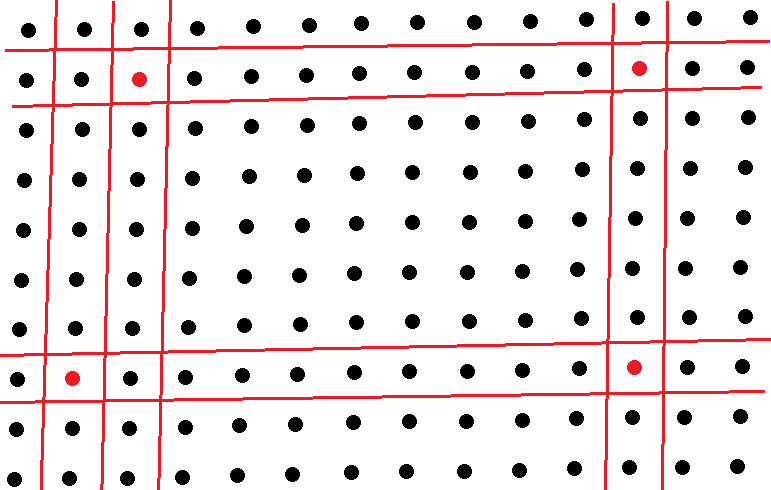
\includegraphics[width=8cm]{skogsbrand_2.png}
\end{center}
\end{figure}


